\documentclass[a4paper,10pt,twocolumn]{ltjarticle}
\usepackage{kaitoushu}

% グラフ用の共通スタイル定義
\pgfplotsset{
  myaxis/.style={
    axis lines=middle,
    xlabel={$x$}, ylabel={$y$},
    every axis x label/.style={at={(ticklabel* cs:1)},anchor=west},
    every axis y label/.style={at={(ticklabel* cs:1)},anchor=south},
    tick label style={font=\scriptsize},
    label style={font=\small},
    width=5.5cm, height=5cm,
    grid=none,
    samples=100,
  }
}

\begin{document}

\problemrange{3章：関数とグラフ — Check (p.33)（問156--164）}



\mondai{156}{放物線 $y=\dfrac{1}{2}x^{2}$ を$x$軸方向に$-2$，$y$軸方向に$1$平行移動した放物線の方程式を求めよ．}
\kotae{
$y=\dfrac{1}{2}(x+2)^{2}+1$
}

\mondai{157}{2次関数 $y=x^{2}+3x$ を標準形に直せ．また，軸と頂点の座標を求め，グラフをかけ．}
\kotae{
$y=\left(x+\dfrac{3}{2}\right)^{2}-\dfrac{9}{4}$

軸：$x=-\dfrac{3}{2}$，頂点：$\left(-\dfrac{3}{2},-\dfrac{9}{4}\right)$

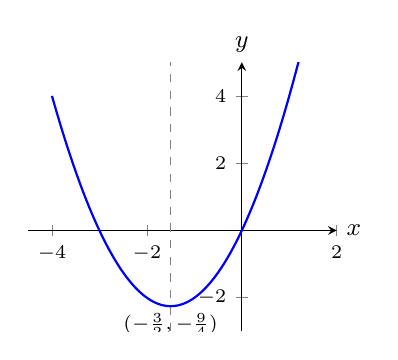
\begin{tikzpicture}
\begin{axis}[myaxis, xmin=-4.5,xmax=2,ymin=-3,ymax=5]
\addplot[thick,blue,domain=-4:1.2]{x^2+3*x};
\node[font=\scriptsize] at (axis cs:-1.5,-2.8) {$(-\frac{3}{2},-\frac{9}{4})$};
\addplot[dashed,gray] coordinates {(-1.5,-3)(-1.5,5)};
\end{axis}
\end{tikzpicture}
}

\mondai{158}{次の条件を満たし，$y$軸に平行な軸をもつ放物線の方程式を求めよ．}
\kotae{
(1) 頂点$(2,-5)$，$(0,7)$を通る → $a=3$．$y=3(x-2)^{2}-5$

(2) 軸$x=-1$，$(0,1)$，$(-3,7)$ → $a=2$，$q=-1$．$y=2(x+1)^{2}-1$

(3) 3点$(1,0)$，$(0,1)$，$(2,3)$ → $a=2$，$b=-3$，$c=1$．$y=2x^{2}-3x+1$
}

\mondai{159}{放物線 $y=x^{2}+2x-3$ を次のように移動した放物線の方程式を求めよ．}
\kotae{
(1) $y$軸対称（$x\to-x$）：$y=x^{2}-2x-3$

(2) 原点対称（$x\to-x$，$y\to-y$）：$y=-x^{2}+2x+3$
}

\mondai{160}{放物線 $y=-x^{2}+6x+1$ は，放物線 $y=-x^{2}-2x+3$ をどのように平行移動したものか．}
\kotae{
頂点の移動を調べる．$(-1,4)\to(3,10)$

$\therefore$ $x$軸方向に$4$，$y$軸方向に$6$平行移動
}

\mondai{161}{2次関数 $y=-x^{2}+4x+1=-(x-2)^{2}+5$ について，次の定義域における最大値と最小値を求めよ．}
\kotae{
(1) $-1\leqq x\leqq 1$：頂点域外．$x=-1$：$-4$，$x=1$：$4$

最小値 $-4$，最大値 $4$

(2) $1\leqq x\leqq 3$：頂点域内．$x=1,3$：$4$，$x=2$：$5$

最小値 $4$，最大値 $5$
}

\mondai{162}{幅16\,cmの鋼板で雨どいを作る．断面積を最大にする折り曲げ幅を求めよ．}
\kotae{
$S=x(16-2x)=-2(x-4)^{2}+32$ → $x=4$\,cm
}

\mondai{163}{$y=x^{2}-6x-k$ と$x$軸の関係．$D=36+4k$}
\kotae{
(1) 2点：$k>-9$\quad (2) 接する：$k=-9$\quad (3) 共有点なし：$k<-9$
}

\mondai{164}{次の2次不等式を解け．}
\kotae{
(1) $(2x+1)(x-2)\leqq0$ → $-\dfrac{1}{2}\leqq x\leqq 2$

(2) $(x+4)^{2}\geqq0$ → すべての実数

(3) $D<0$，常に正 → 解なし
}

\end{document}
